\newpage
{\large\textbf{Graphs}}
\begin{figure}[H]
    \centering
	\begin{subfigure}{0.45\textwidth}
		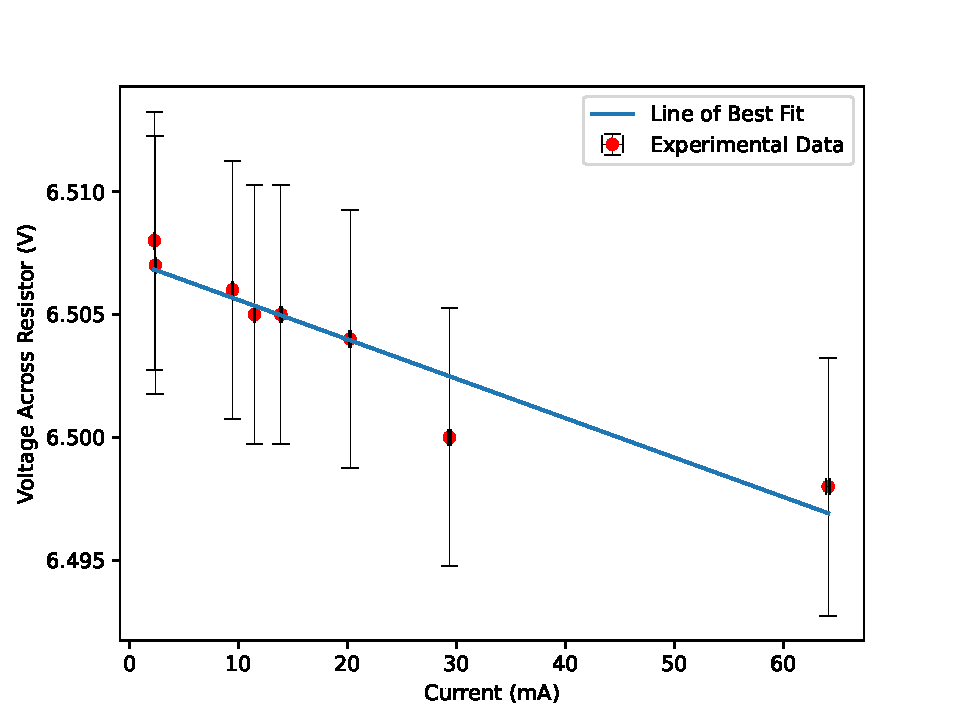
\includegraphics[width=\textwidth]{graph1}
		\caption{\textbf{Figure 3: Measured Voltage vs Measured Current for the circuit denoted in setup 1. The current and voltage measurements are taken at the locations of the respective detector in the schematic. The voltage source is the battery. The negative of the slope is the output resistance value.}}
	\end{subfigure}
    \hspace{0.08\textwidth}
	\begin{subfigure}{0.45\textwidth}
		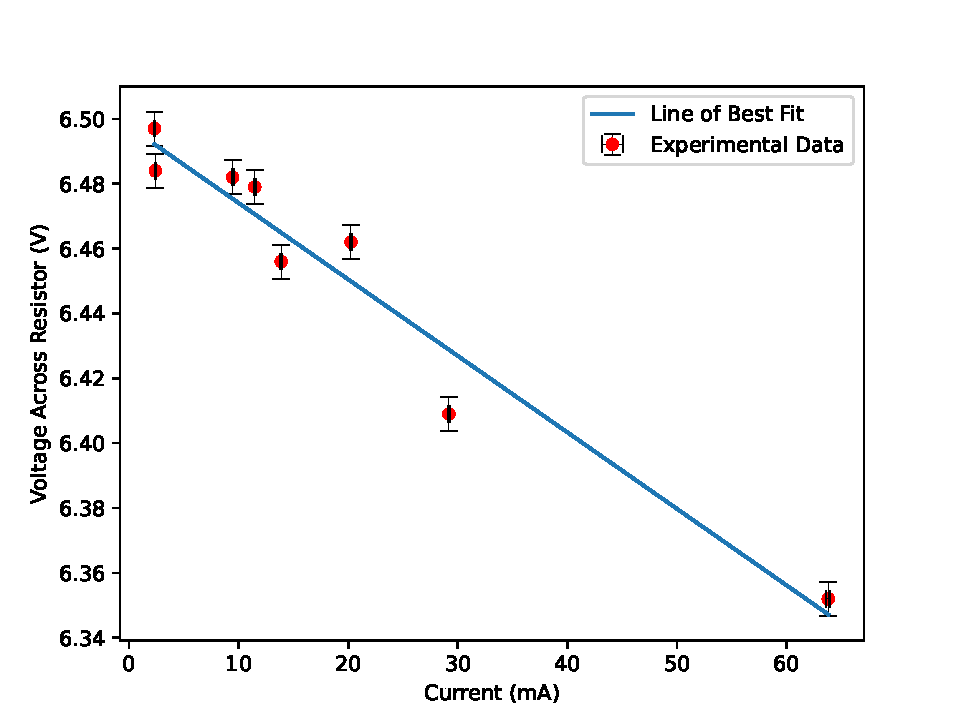
\includegraphics[width=\textwidth]{graph2}
		\caption{\textbf{Figure 2: Measured Voltage vs Measured Current for the circuit denoted in setup 2. The current and voltage measurements are taken at the locations of the respective detector in the schematic. The voltage source is the battery. The negative of the slope is the output resistance value.}}
	\end{subfigure}
    \begin{subfigure}{0.45\textwidth}
		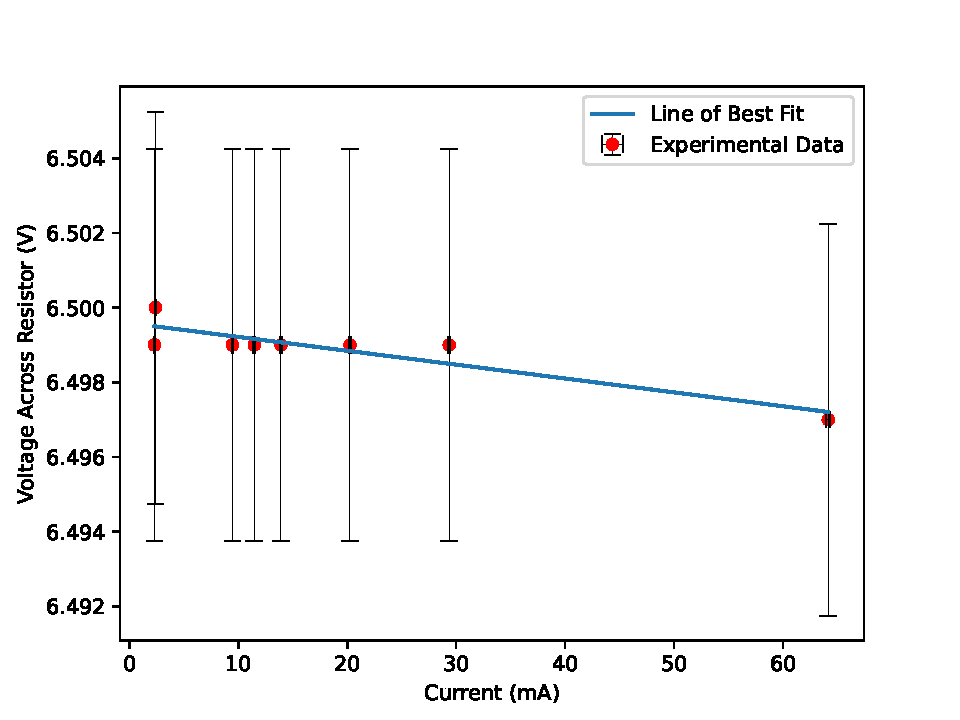
\includegraphics[width=\textwidth]{graph3}
		\caption{\textbf{Figure 3: Measured Voltage vs Measured Current for the circuit denoted in setup 1. The current and voltage measurements are taken at the locations of the respective detector in the schematic. The voltage source is the regulated power supply set at 6.5V. The negative of the slope is the output resistance value.}}
	\end{subfigure}
    \hspace{0.08\textwidth}
	\begin{subfigure}{0.45\textwidth}
		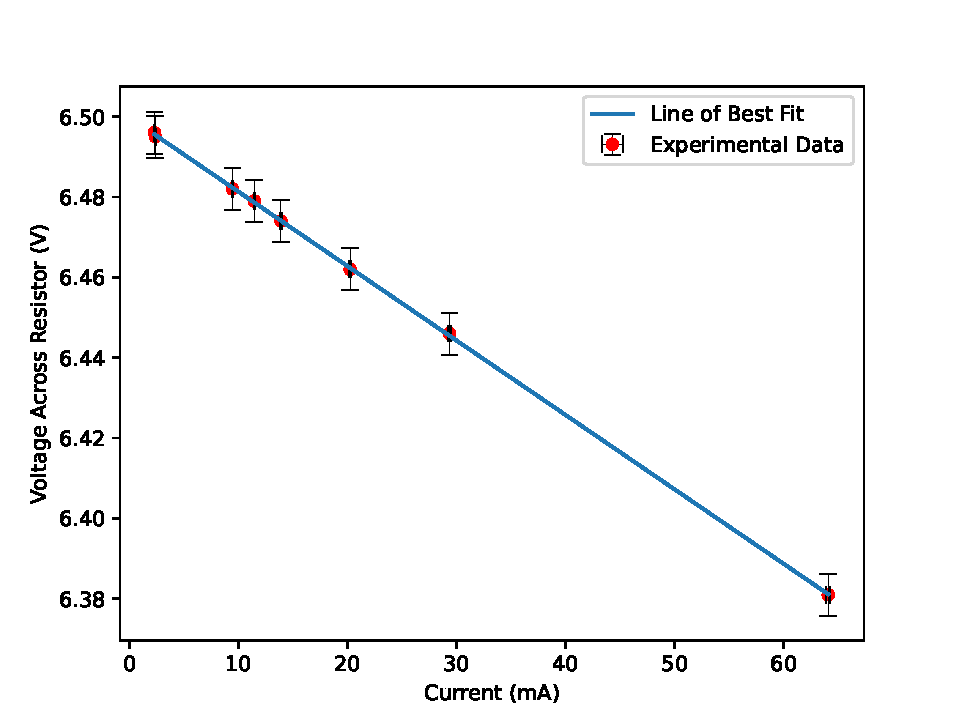
\includegraphics[width=\textwidth]{graph4}
		\caption{\textbf{Figure 4: Measured Voltage vs Measured Current for the circuit denoted in setup 2. The current and voltage measurements are taken at the locations of the respective detector in the schematic. The voltage source is the regulated power supply set at 6.5V. The negative of the slope is the output resistance value.}}
	\end{subfigure}

\end{figure}

\begin{figure}[H]
    \centering
    \begin{subfigure}{0.45\textwidth}
		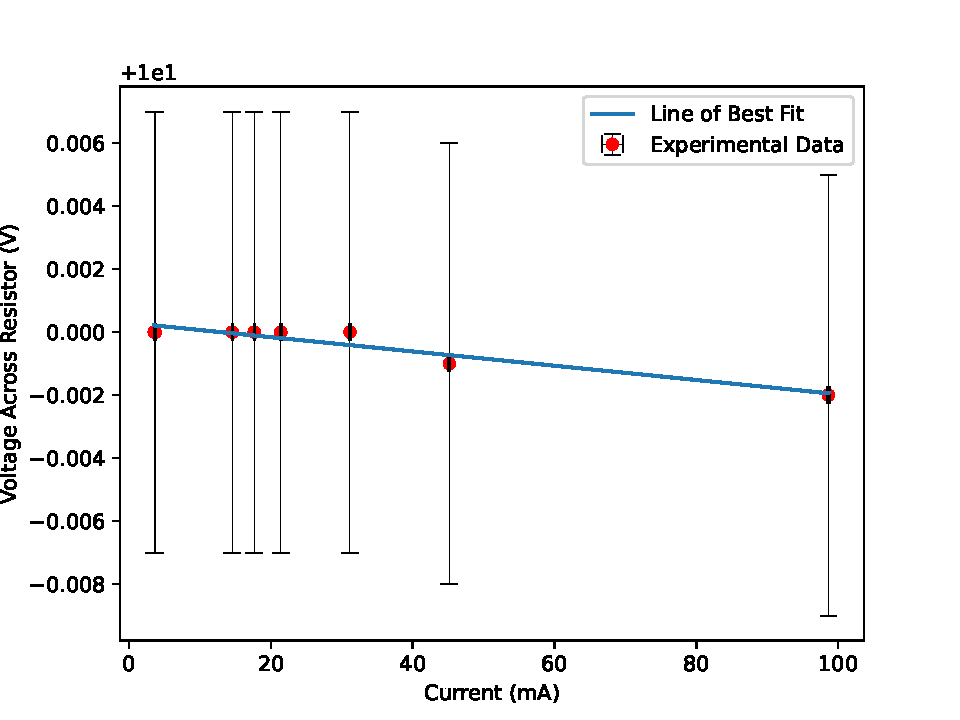
\includegraphics[width=\textwidth]{graph5}
		\caption{\textbf{Figure 5: Measured Voltage vs Measured Current for the circuit denoted in setup 1. The current and voltage measurements are taken at the locations of the respective detector in the schematic. The voltage source is the regulated power supply set at 10V. The negative of the slope is the output resistance value.}}
	\end{subfigure}
    \hspace{0.08\textwidth}
	\begin{subfigure}{0.45\textwidth}
		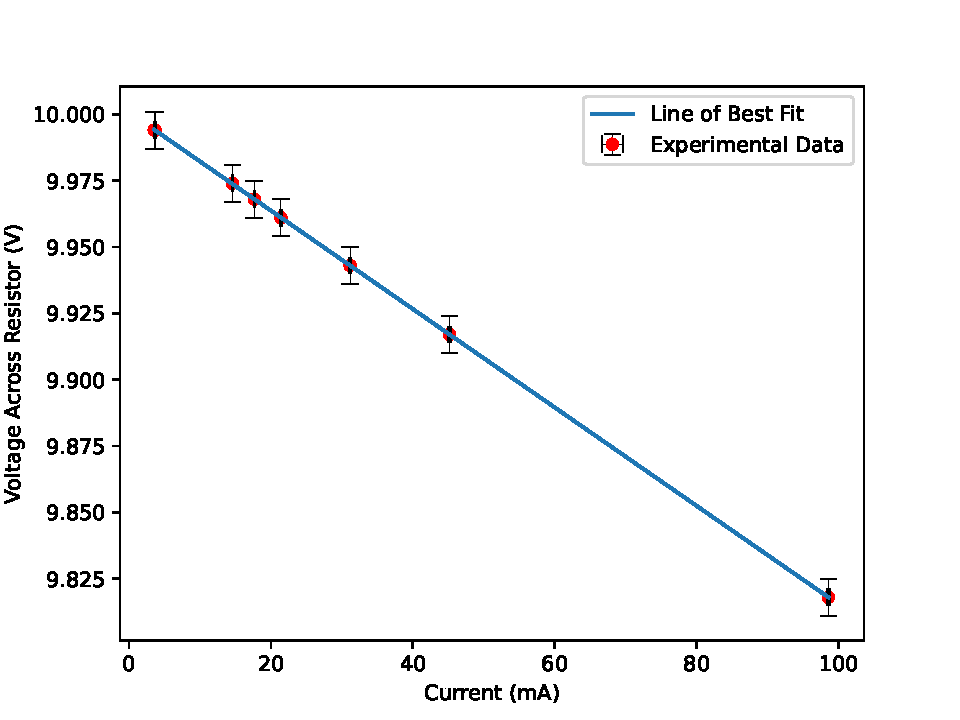
\includegraphics[width=\textwidth]{graph6}
		\caption{\textbf{Figure 6: Measured Voltage vs Measured Current for the circuit denoted in setup 2. The current and voltage measurements are taken at the locations of the respective detector in the schematic. The voltage source is the regulated power supply set at 10V. The negative of the slope is the output resistance value.}}
	\end{subfigure}
    \begin{subfigure}{0.45\textwidth}
		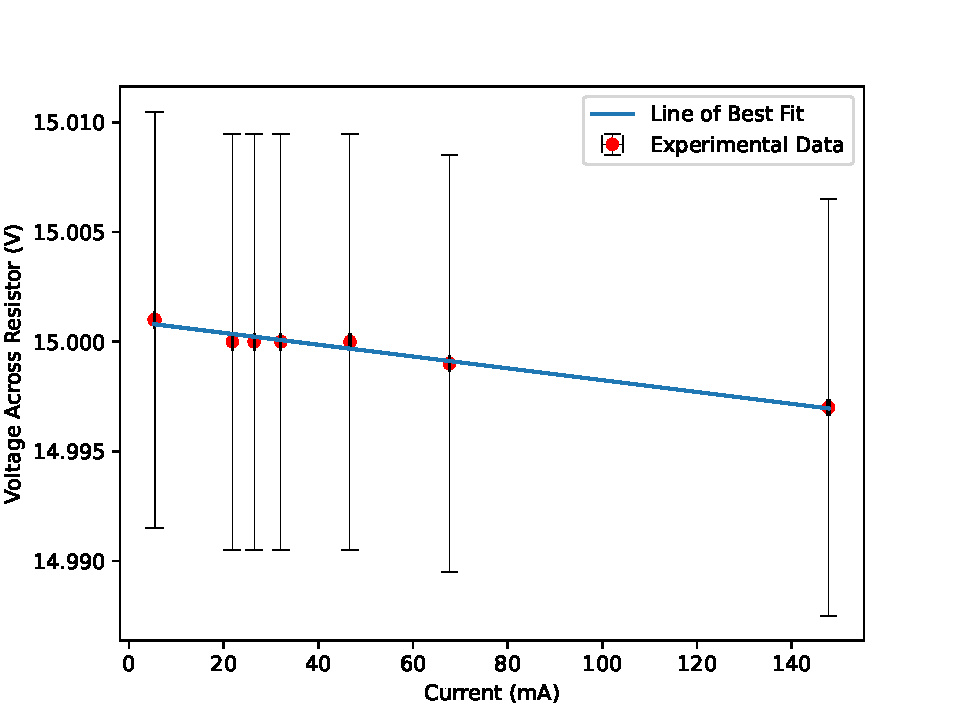
\includegraphics[width=\textwidth]{graph7}
		\caption{\textbf{Figure 7: Measured Voltage vs Measured Current for the circuit denoted in setup 1. The current and voltage measurements are taken at the locations of the respective detector in the schematic. The voltage source is the regulated power supply set at 15V. The negative of the slope is the output resistance value.}}
	\end{subfigure}
    \hspace{0.08\textwidth}
	\begin{subfigure}{0.45\textwidth}
		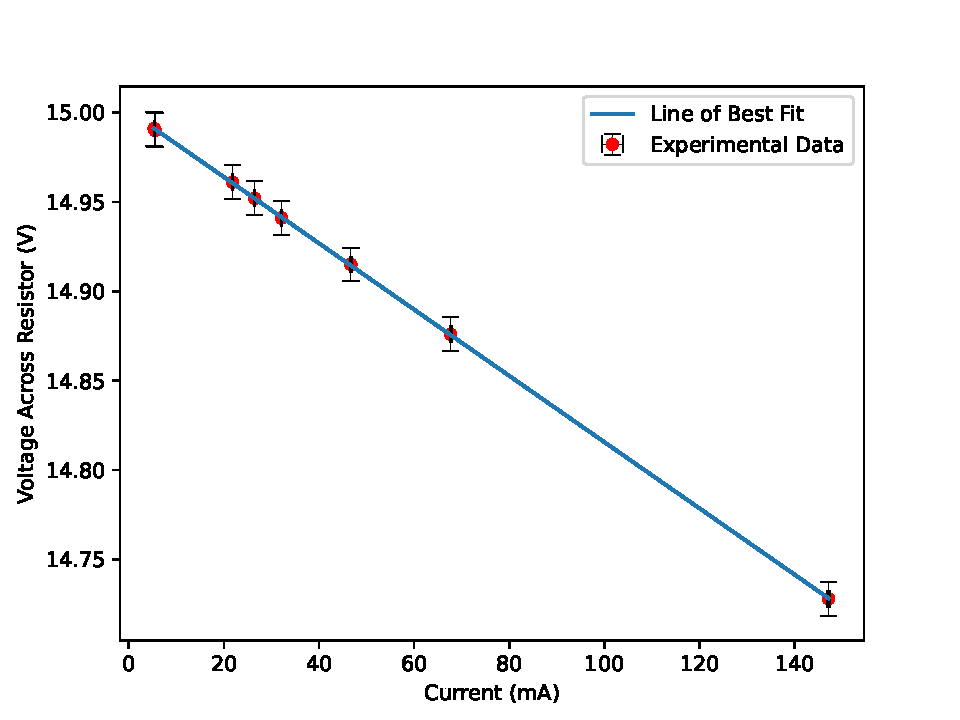
\includegraphics[width=\textwidth]{graph8}
		\caption{\textbf{Figure 8: Measured Voltage vs Measured Current for the circuit denoted in setup 2. The current and voltage measurements are taken at the locations of the respective detector in the schematic. The voltage source is the regulated power supply set at 15V. The negative of the slope is the output resistance value.}}
	\end{subfigure}
\end{figure}

\begin{figure}[H]
	\begin{subfigure}{0.45\textwidth}
		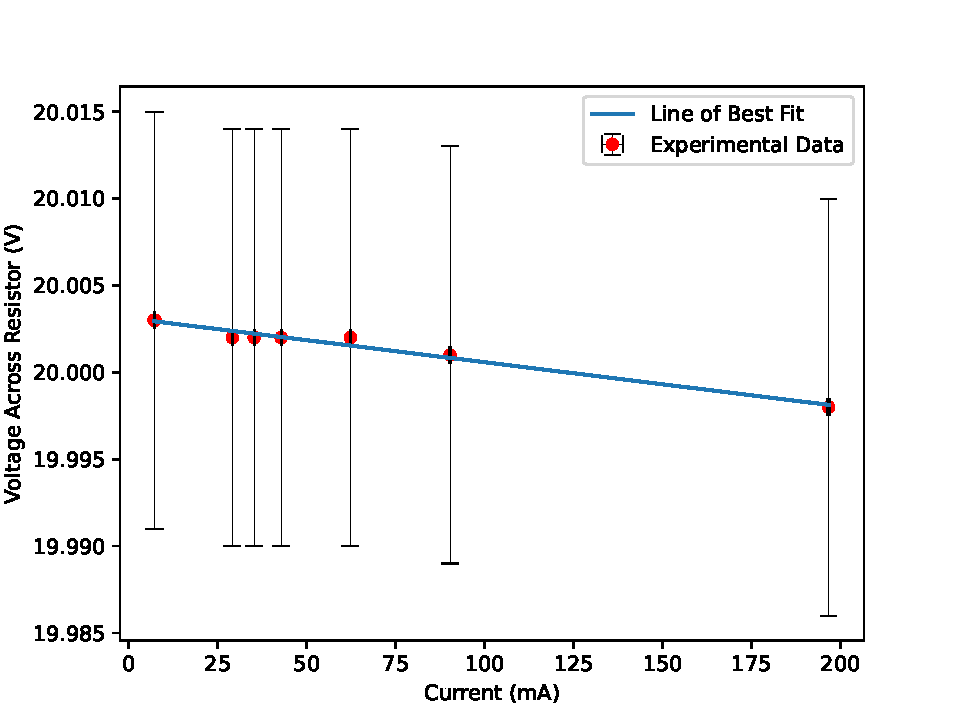
\includegraphics[width=\textwidth]{graph9}
		\caption{\textbf{Figure 9: Measured Voltage vs Measured Current for the circuit denoted in setup 1. The current and voltage measurements are taken at the locations of the respective detector in the schematic. The voltage source is the regulated power supply set at 20V. The negative of the slope is the output resistance value.}}
	\end{subfigure}
    \hspace{0.08\textwidth}
	\begin{subfigure}{0.45\textwidth}
		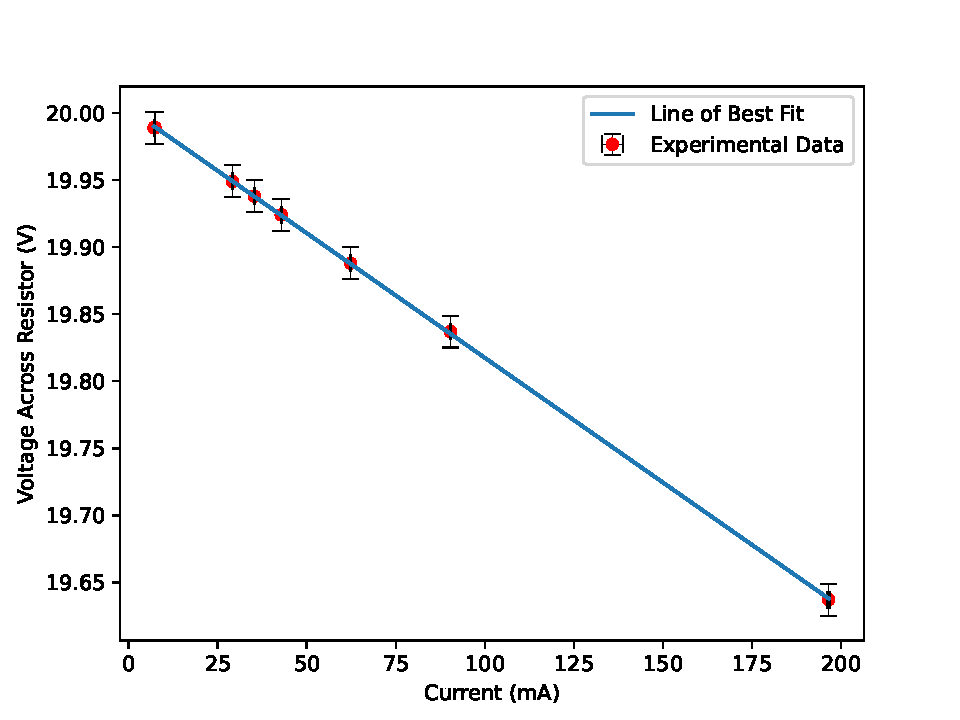
\includegraphics[width=\textwidth]{graph10}
		\caption{\textbf{Figure 10: Measured Voltage vs Measured Current for the circuit denoted in setup 2. The current and voltage measurements are taken at the locations of the respective detector in the schematic. The voltage source is the regulated power supply set at 20V. The negative of the slope is the output resistance value.}}
	\end{subfigure}
    \begin{subfigure}{0.45\textwidth}
		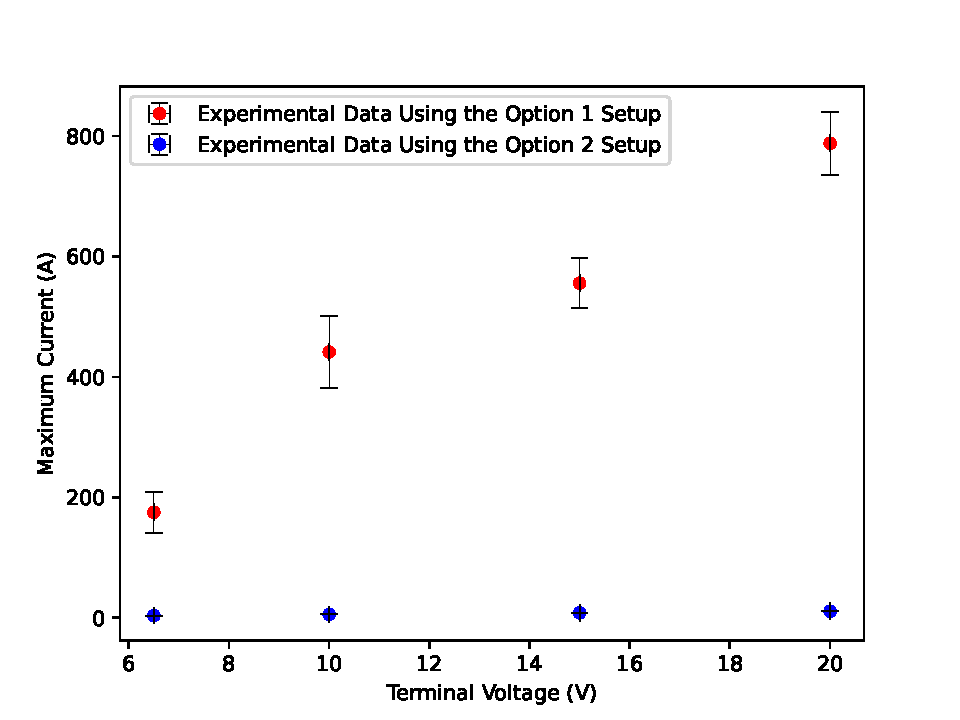
\includegraphics[width=\textwidth]{maxCurrent}
		\caption{\textbf{Figure 11: Graph demonstrating the relationship between maximum current and terminal voltage, varying linearly on one another.}}
	\end{subfigure}
\end{figure}
